\section{Gnuplot}\label{sec:gnuplot}

Gnuplot é uma ferramenta gratuita capaz gerar gráficos a partir de funções matemáticas de duas ou três dimensões, e conjuntos de dados \cite{gnuplot5Doc}.

A geração de gráficos pode ocorrer diretamente na tela do computador ou ser direcionada para arquivos de diversos formatos, tais como JPEG, PNG, EPS e SVG. A criação automatizada de códigos LaTeX\footnote{Conjunto de macros para a confecção de textos Tex amplamente utilizada no meio acadêmico, principalmente por matemáticos, físicos e cientistas da computação.} é suportada, permitindo a inclusão simplificada diretamente nos documentos escritos nessa linguagem \cite{gnuplot5Doc}. 

Como visto em \cite{gnuplot5Doc}, o programa pode ser usado tanto interativamente, por meio de linhas de comando, quanto através de scripts em lote (batch mode). As figuras \ref{gnu_sincos} e \ref{gnu_sincos_code} apresentam um exemplo de gráfico gerado pela ferramenta e o seu código, respectivamente.

\begin{figure}[htp!]
\centering
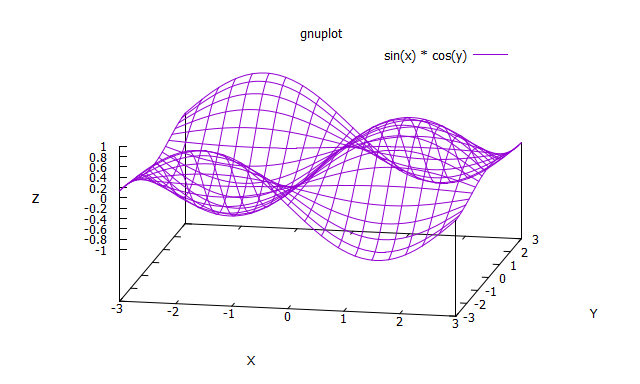
\includegraphics[width=1\textwidth]{figuras/cap_3/secao_3/gnuplot_sincos.png}
\caption{Gráfico gerado utilizando o gnuplot para a função $sin(x) . cos(y)$}
\label{gnu_sincos}
\end{figure}

\begin{figure}[htp!]
\centering
\lstinputlisting[language=gnuplot]{codigos/gnuplot.gnu}
\caption{Script utilizado para a geração do gráfico da figura \ref{gnu_sincos}}
\label{gnu_sincos_code}
\end{figure}

Dentro do contexto do trabalho, a utilização da ferramenta auxilia na geração de gráficos contendo os resultados dos testes, feitos por meio do simulador the ONE, e da análise dos resultados apresentados por meio de gráficos.